\section{Architecture and Implementation}
\label{sec:architecture}

%%%%%%%%%%%%%%%%%%%%%%%%%%%%%%%%%%%%%%%%%%%%%%%%%%%%%%%%%%%%%%%%%%%%%%%%%%%%%%%%%%%%%%%
% Intro to arch
%%%%%%%%%%%%%%%%%%%%%%%%%%%%%%%%%%%%%%%%%%%%%%%%%%%%%%%%%%%%%%%%%%%%%%%%%%%%%%%%%%%%%%%

To simplify and address concerns outlined in the previous section we introduce two
major changes. We introduce safe collections, an abstraction that encapsulates
a data-set and the set of policies that govern its use. Seconondly, in order to separate
administative responsibilities pertaining to the safe-collection from the infrastructure
admins, we create a new class of privileged users called Stewards. In this model, administrators
create a safe collection and hand over all administrative privileges to the stewards. This transfers
all administrative responsibilities regarding access and export of data to the stewards who now take
ownership and responsibility for the safe collection.

\subsection{Safe Collection}

Data-sets come with various levels of sensitivity and selecting the protocols to ensure adequate security
requires a case-by-case treatement. To closely integrate such policies with the data-set we have created
safe-collections. Safe collections allows the system administrators to partition the key administration
aspects of managing the relationship between analysts and a data to experienced curators of the data-set.
Safe-collections encapsulate a data-store where the dataset will reside, and a consistent set of policies
that controls access to data-store as well the policies themselves.

Since our existing production systems are built on Amazon Web Services(AWS), we have extended our work by
leverage services and guarantees provided by AWS. The data-store is implemented over S3 object store, and the
policies are implemented as Identity and Access Management(IAM) policies and S3 bucket policies.
A safe-collection is described in cloudformation, a JSON based software defined infrastructure system for AWS.
This allows our safe-collection descriptions to be reproducible and shareable.

Safe-collections enable the specification of limits and controls on access, usage and export of data.
The initial specification is a meta policy that defines the set of policies permissible on a safe-collection and
a steward group permitted to update the access policies. This meta policy schema translates to a form
at the creation of the safe-collection and is implemented as tags on the data-store. The schema is enforced
by the various services that interact with the safe-collection. The schema and the generated form are shown in
\figurename~\ref{fig:schema}

\begin{figure*}[ht]
  \center
  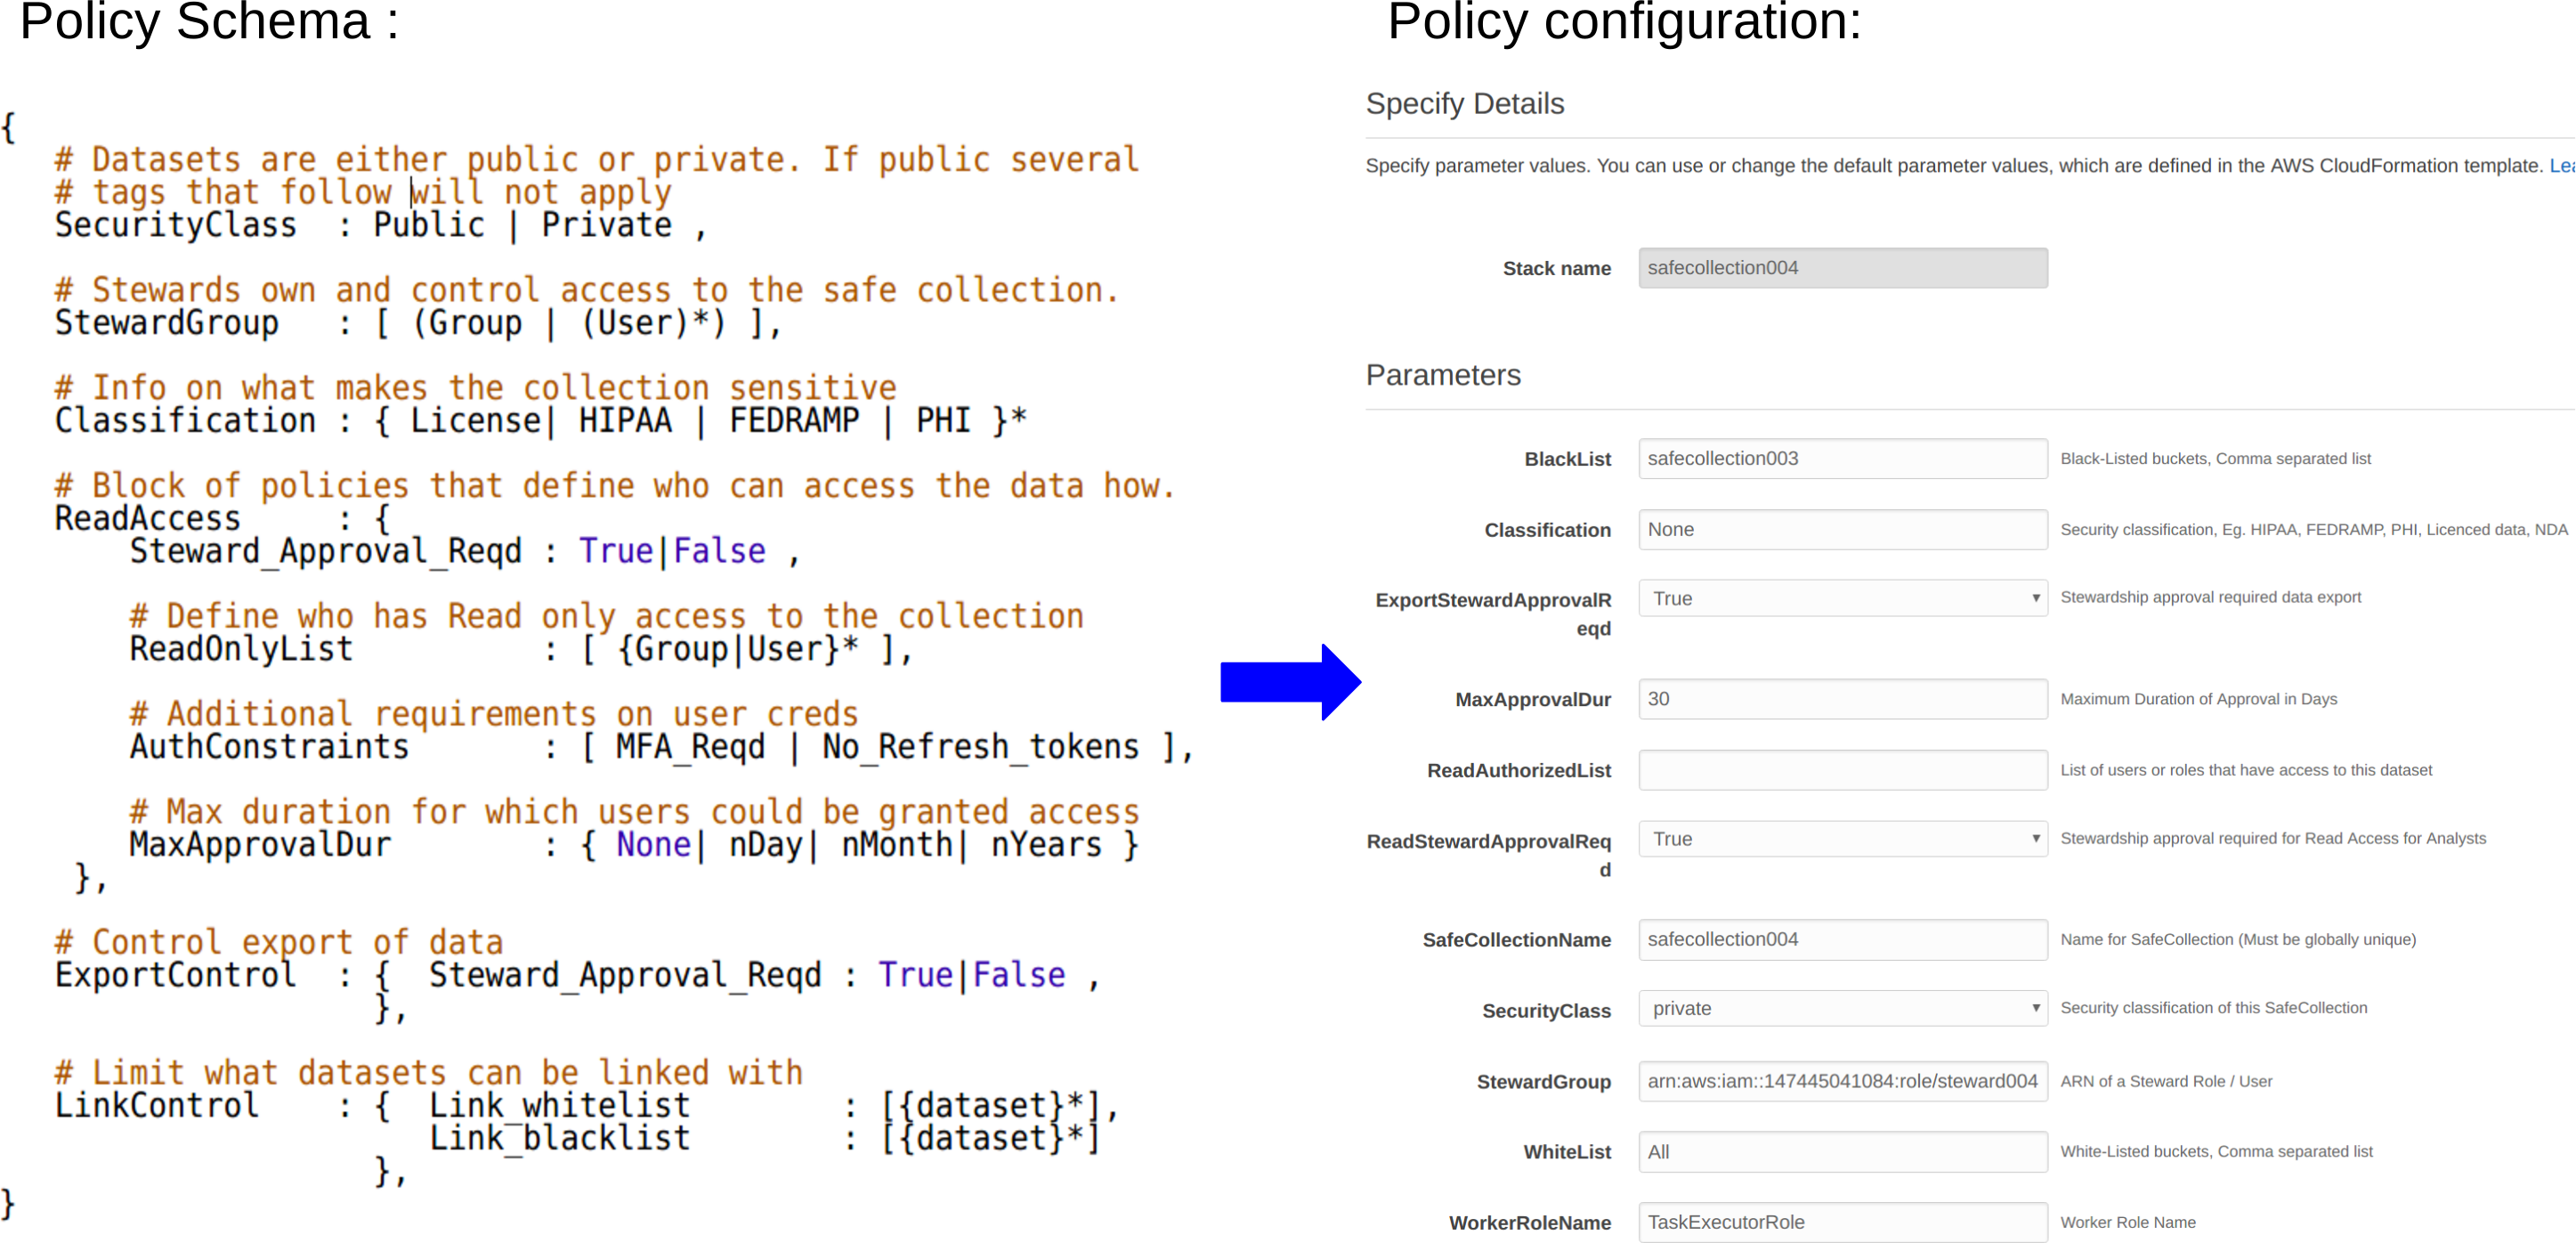
\includegraphics[width=\textwidth, height=8cm]{figures/meta-policy.png}
  \caption{Meta-policy specification and configuration}
  \vspace{-1.5em}
  \label{fig:schema}
\end{figure*}

% Public data
Public data-sets are assumed to contain no sensitive content and thus do not require access control nor
export control. Setting \texttt{SecurityClass} to \texttt{Public} indicates that the safe-collection does
not require a Steward and that all authenticated users on \NAME may access this dataset. None of the added
security features of safe-collections need apply.

% Common features for private data
Confidential and regulated datasets both require \texttt{SecurityClass} to be set to \texttt{Private}
and require that a steward group is specified. In addition, constraints can be set on the duration
for which analysts could be granted access. This ensures that access privileges expire and require
re-evaluation of the scope and nature of the analyst's work before access is extended. To limit the risk of
re-identification in datasets that contain anonymized data the safe-collections allow for whitelisting and
blacklisting other safe-collections. Job submissions to \NAME are checked for data requests that have
linkage conflicts, and denied at submit time.
\yadu{Linkage feature pending}

% implementation of access control
Access control on safe-collections for private datasets are managed by stewards. Access privileges to
safe-collections are granted, extended and revoked via S3 bucket policies. At the time of creation all
privileges over bucket policies are granted to the steward and revoked for all other entitites. This
guarantees that only the stewards can grant privileges on safe-collection. Access is granted by stewards
by adding a new bucket policy conditional on an expiration deadline. These policies may be revoked or
extended by updating the expiration deadline, thus offering fine-grained control to stewards on managing
access.

% cite garfinkel for de-identification risks

Safe-collections that contain regulated datasets often require oversight to ensure that all computed results
are inspected and approved by a steward before export. This is enforced by setting the
\texttt{ExportStewardApprovalReqd} flag.
Analysis results from tasks that consumed data from any safe-collection with this flag has all of the
results posted back to the same safe-collection, thus inheriting the same privileges as the source.
% worker roles are granted write privileges to the outputs section of a safe-collection
As a result, only stewards can view the results and export to a public safe-collection. Since results are
stored within the parent safe-collection, users can apply analysis operations on results without oversight,
and only request for export of the final results of a deep analysis pipeline.

\subsection{Stewardship}

% Why do we have them / inital role
As more data-sets with varying degrees of sensitivity are added to the \NAME platform it becomes a matter
of necessity to distribute key administrative privileges from the system administrator roles to the curators
of the data-set. Stewards play a leadership role in evaluating the disclosure risks associated with a
dataset and codifying the security protocols protecting the safe-collection.

% implementation details
Upon creation of a safe-collection a single steward group implemented as an IAM role, is added to the
access policies of the safe-collection. This steward role is the sole entity on the platform capable of
updating polices attached to the safe-collection.
Multiple users could be associated with a steward role and is recommended, so that requests can be served quicker.
Once user identities are established by authenticating with an external identity provider,
\NAME allows users to ``assume'' a privileged IAM role that they have been attached to.
By assuming the steward role, a user temporarily gains the privileges to carry out operations such
as updating access policies and exporting data from a safe-collection.
Once created the steward's responsibilities are two-fold: arbitrate access requests to the safe-collection and
handle export requests for results generated from safe-collections.

% access
Analysts can list all available safe-collections and request access to ones that they require.
Stewards evaluate these requests and approve access for a duration. Approvals are implemented as an additional
policy added to the list of s3 bucket policies for the safe-collection. \NAME ensures that the policy
being added is consistent with the meta-policy for the safe-collection, for eg. expiration for the policy
must be within the duration specified in the \texttt{MaxApprovalDur}.
\yadu{pending}

% export
On export controlled safe-collections, results generated by analysis tasks on \NAME are not visible to the
analysts until approved by a Steward. This is implemented by having workers write all results to the
parent safe-collections output directory and thus inheriting the same security privileges of the parent.
On \NAME stewards have complete visibility over the set of inputs, and operations made by the analysts
in order to generate their results. It is also possible to trace the provenance of the results from an
analysis pipeline since all analysis tasks are logged.
Stewards export the results by transferring the results out of the safe-collection and onto a public
safe-collection from which analysts can view results. It is important to note that even public
safe-collections have server side encryption and are only accessible to authenticated users via temporary
signed urls.


\subsection{User Flows}

Here we will look at the two most common flows introduced by this model:

\subsubsection{Access Flow}

\begin{itemize}
\item request access
\item grant access
\item submit job
\item fetch data
\item compute
\item store results
\end{itemize}

\subsubsection{Export Flow}

\begin{itemize}
\item Export request
\item Initiate export
\item Export data
\item Access results
\end{itemize}




%\begin{figure}
%  \center
%  %\includegraphics[width=0.45\textwidth]{figures/arch.pdf}
%  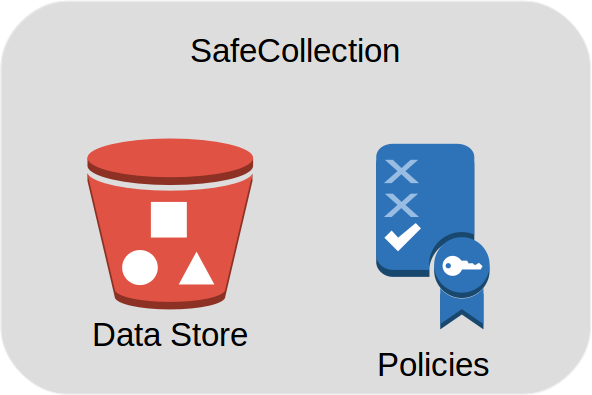
\includegraphics[width=0.45\textwidth]{figures/safecollection.png}
%  \caption{Safe collection schema}
%  \label{fig:safe_schema}
%  \vspace{-1.5em}
%\end{figure}

\begin{figure}
  \center
  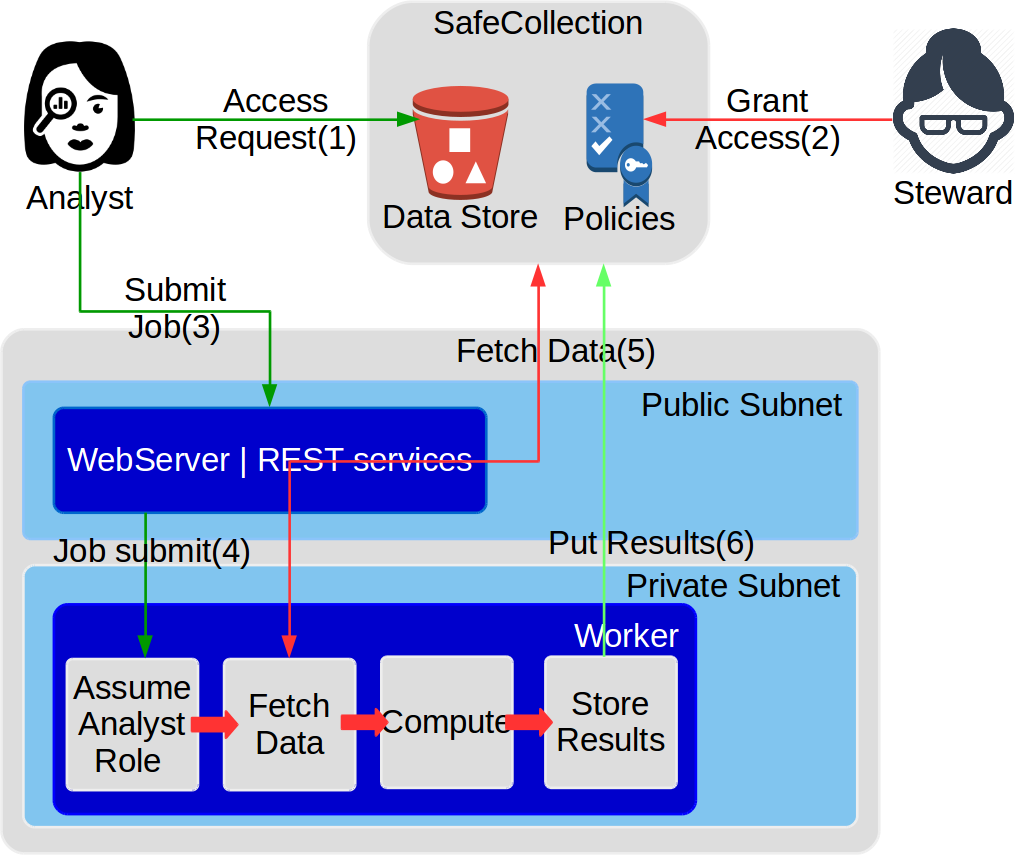
\includegraphics[width=0.45\textwidth]{figures/safe_flow.png}
  \caption{Safe collection schema}
  \label{fig:flow1}
  \vspace{-1.5em}
\end{figure}


\begin{figure}
  \center
  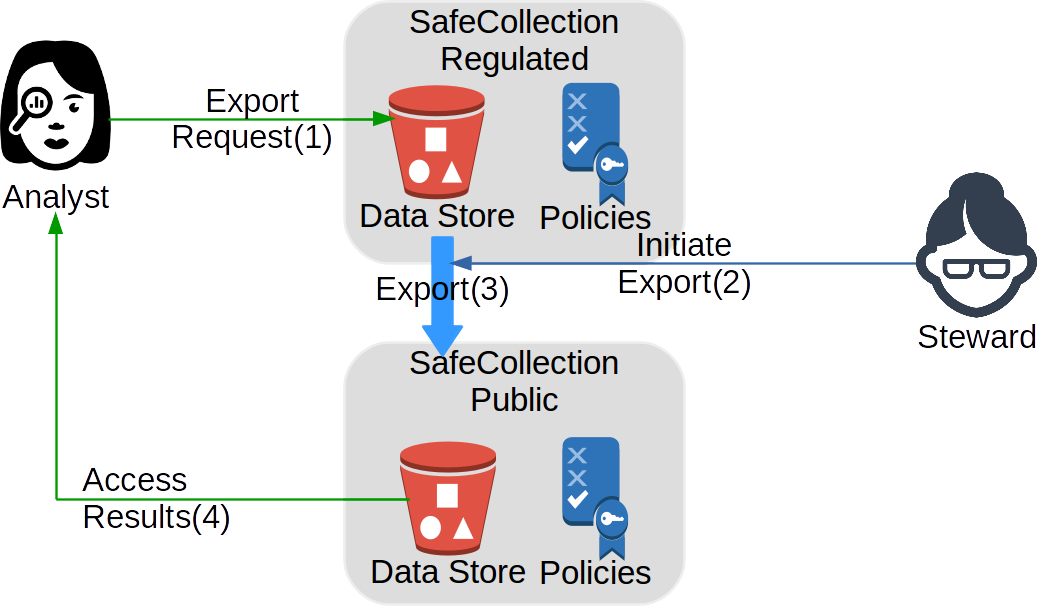
\includegraphics[width=0.45\textwidth]{figures/export_flow.png}
  \caption{Safe collection schema}
  \label{fig:flow2}
  \vspace{-1.5em}
\end{figure}









